% Structured Outputs Do Not Imply Compatible Uncertainty
% Build: pdflatex main && bibtex main && pdflatex main && pdflatex main
% (or: latexmk -pdf main; or: tectonic main.tex). Figure data: python3 make_figure_data.py
\documentclass[11pt]{article}

\usepackage[margin=1in]{geometry}
\usepackage[T1]{fontenc}
\usepackage{lmodern}
\usepackage{microtype}
\usepackage{amsmath,amssymb}
\usepackage{booktabs}
\usepackage{tabularx}
\usepackage{multirow}
\usepackage{xcolor}
\usepackage{tikz}
\usetikzlibrary{arrows.meta,positioning}
\usepackage{pgfplots}
\pgfplotsset{compat=1.17}
\usepgfplotslibrary{groupplots}
\usepackage[numbers,sort&compress]{natbib}
\usepackage[hidelinks]{hyperref}
\usepackage[capitalise]{cleveref}

\newcolumntype{Y}{>{\raggedright\arraybackslash}X}
\newcommand{\choice}{\texttt{choice}}
\newcommand{\noul}{\texttt{noul}}
\newcommand{\score}{\texttt{score}}
\newcommand{\astar}{a^{*}}

\title{Structured Outputs Do Not Imply Compatible Uncertainty:\\
An Empirical Study of Confidence Signals in a Multi-Step Decision Workflow}

% Anonymous for review. Contributors: see repository history.
\author{Anonymous Authors}
\date{}

\begin{document}
\maketitle

\begin{abstract}
Structured-output decision APIs return well-typed answers together with
numeric confidence, and it is tempting to treat those numbers as
interchangeable probabilities that can be composed across the steps of a
workflow. We examine that practice for the three decision primitives of
one commercial API: a categorical \choice{}, a binary \noul{} and an
ordinal \score{}. The primitives are chained into a three-step triage
workflow (route, assess, rate severity). We evaluate on controlled
constructed items, on 202 Mozilla bugs labeled by triage and on 240 Linux
kernel bugs labeled by their reporters, using 4{,}584 API calls in the main
real-data runs. Three findings hold on both trackers.
First, the primitives' confidence signals have distinct failure modes.
\choice{} confidence is saturated (85--96\% of real bugs at $\geq 0.90$)
yet discriminative (AUROC 0.90 [0.83, 0.96] and 0.98 [0.95, 1.00]).
\noul{}'s confidence-like value is uninformative (AUROC 0.53
[0.42, 0.65] and 0.41 [0.32, 0.50]). \score{}'s confidence is flat across
true severity levels.
Second, fixed confidence thresholds designed on constructed data lose
their intended selectivity on real text: a cut that escalated 73\% of
constructed items (target 67\%) escalated 88\% and 78\% of real bugs
(targets 41--42\%).
Third, \score{} compresses severity toward the middle level, consistent
with central-tendency bias reported for LLM raters in other domains, and
its confidence gives no indication of it.
In exploratory analyses, the composition rules we tested did not
consistently identify which cases to escalate: ranking escalations by
composed confidence was indistinguishable from random selection on both
trackers, although the intervals cannot exclude a modest signal. We
also show that a natural comparison of confidence-based against
decision-based composition is confounded when the target action is
itself a function of the decisions. The corrected comparison is
pre-registered for a controlled follow-up that has not yet been run.
\end{abstract}

%======================================================================
\section{Introduction}
%======================================================================

A model can return a perfectly valid, well-typed structured response and
still make the wrong decision. When several such decisions are chained
into a workflow, errors at one step propagate to the next. A common hope
is that each step's reported confidence can be composed into a
workflow-level signal that says when to hand a case to a human.

We ask a narrower and more testable question. \emph{When a workflow
chains heterogeneous decision primitives, can it rely on their
uncertainty signals, and how should it combine them?} Heterogeneity
matters because the API we study exposes three primitives whose
uncertainty is \emph{structurally} different. \choice{} returns a
distribution over labels plus a scalar confidence. \score{} returns an
ordinal distribution plus a scalar confidence. \noul{} returns a single
probability with no separate confidence field. Treating these numbers as
one kind of quantity is a modeling assumption, and this paper tests it.

\paragraph{Contributions.}
\begin{enumerate}
  \item \textbf{Characterization} (\cref{sec:char}). Per-primitive behavior
  of confidence on controlled and real data, showing three incompatible
  profiles.
  \item \textbf{Transfer} (\cref{sec:transfer}). Fixed thresholds set on
  constructed content lose their selectivity on real text, in two
  distinct ways.
  \item \textbf{Real-data validation} (\cref{sec:real}). Two bug trackers
  from different projects, with different labeling processes (triage and
  reporter), on which severity compression appears in both.
  \item \textbf{Composition} (\cref{sec:comp}, exploratory). The
  confidence-based escalation rules we tested did not consistently pick
  better cases than random on either tracker. We identify, and correct for
  the follow-up, a confound in the obvious comparison.
  \item \textbf{Method} (\cref{sec:method}). A pre-registration and audit
  process that caught six design or implementation defects, most of them
  before any evaluation data existed.
\end{enumerate}

\paragraph{Non-claims.} We make no claim about general calibration, other
APIs or model versions, domains beyond software bug triage, or real-world
operational benefit.

%======================================================================
\section{Related work}
%======================================================================

\paragraph{Calibration of single decisions.} Post-hoc calibration
\citep{platt1999probabilistic,naeini2015bbq} and the miscalibration of
modern networks \citep{guo2017calibration} are well studied, and
confidence estimation for language models has been surveyed in
\citep{geng2024survey}.

\paragraph{Selective prediction and deferral.} Risk--coverage trade-offs
and reject options \citep{elyaniv2010selective,geifman2017selective,geifman2019selectivenet},
learning to defer \citep{madras2018predict} and prediction sets in
human--AI teams \citep{babbar2022predsets} address \emph{one} decision.

\paragraph{Conformal methods and composition.} Conformal prediction
\citep{angelopoulos2021gentle} and conformal risk control
\citep{angelopoulos2024crc} give distribution-free guarantees. Composition
across stages has been studied for two stages \citep{zhang2025modular}
and for multi-stage NLP pipelines, where independently calibrated
per-stage coverage compounds multiplicatively \citep{kotte2026pasc}.
Error propagation through pipeline steps has also been quantified
\citep{chowdhury2019error}. Classical reliability theory composes
component reliabilities \citep{barlow1965reliability}.

\paragraph{Cascades and escalation.} Cascades route a \emph{single} query
through model tiers. Prior work studies early abstention
\citep{zellinger2025early}, decision-theoretic escalation
\citep{bouchard2026escalation}, conformal cascades
\citep{dou2026conformalcascade}, confidence tuning \citep{rabanser2025gatekeeper}
and judges with escalation guarantees \citep{jung2025trust}.

\paragraph{Combining confidence across components.} Fixed combination
rules such as the product rule are classical
\citep{kittler1998combining}. The product rule's usual justification
assumes conditional independence and comparable probability scales, and
these are precisely the assumptions our strategy S2 makes implicitly. At
the system level, a recent taxonomy argues that uncertainty in LLM
applications must be studied across the whole compound system, as it
propagates between model calls, workflow stages and human processes
\citep{xia2026propagation}. Cost-sensitive deferral to multiple experts
under workload limits \citep{alves2024defer} formalizes the budgeted
escalation setting our follow-up uses.

\paragraph{Ordinal outputs and central tendency.} LLM raters have been
reported to compress ordinal scores toward the middle of the scale, for
example in clinical scoring, where prompt changes did not remove the
effect \citep{zhang2026centraltendency}. Few-label calibration of ordinal
LLM outputs models such flattening explicitly \citep{wang2026cordial}.
Our severity result is consistent with this literature. What we add is
that it appears in bug triage, against two labeling processes, and that
the primitive's own confidence gives no sign of it.

\paragraph{Agents and trajectories.} Closest to us, step-level
calibration has been shown not to imply trajectory-level calibration for
LLM agents \citep{lin2026uqagents}. Related work calibrates agent
trajectories \citep{zhang2026agentic} and studies uncertainty propagation
in multi-step agentic decisions \citep{duan2025uprop}.

\paragraph{Positioning.} Prior work studies calibration of single
decisions, cascades of the \emph{same} decision, agent trajectories, and
system-level propagation in general. Our contribution is narrower and
empirical. We measure how the uncertainty signals of three
\emph{structurally different} primitives of one API behave inside one
workflow against real labels, and whether simple composition rules over
them identify escalation candidates. We are not aware of prior work with
this specific design. Our literature search was web-based and did not
systematically cover reliability engineering or HCI escalation
research, so we make no stronger priority claim.

%======================================================================
\section{Setting}
\label{sec:setting}
%======================================================================

\paragraph{Primitives and repeats.} All runs use model version
\texttt{jev-1.13.0}. Each node is called three times, and the three
answers are reduced to one decision. For \choice{} and \score{} we take
the modal decision with a tie tolerance of 0.02; a node with no
two-of-three majority is \emph{repeat-unstable}. For \noul{} we threshold
the mean probability at 0.5, and its confidence-like value is
$2\,|\bar{p}-0.5|$.

\paragraph{Workflow.} Node~1 (\choice{}) routes the incident to a
network or storage subsystem. Node~2 (\noul{}) assesses a binary
property: customer impact on constructed data, regression on real bugs.
Node~3 (\score{}) rates severity on three levels. Each node reads the
evidence plus the upstream decisions, appended by a fixed adapter
(\cref{fig:workflow}).

\begin{figure}[t]
\centering
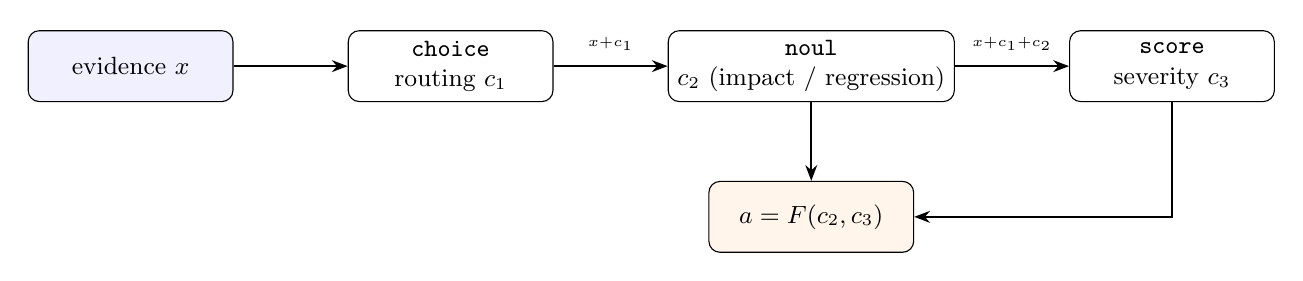
\begin{tikzpicture}[node distance=1.45cm, every node/.style={font=\small},
  box/.style={draw, rounded corners, minimum width=2.6cm, minimum height=0.9cm, align=center},
  arr/.style={-{Stealth[length=2mm]}, thick}]
\node[box, fill=blue!6] (ev) {evidence $x$};
\node[box, right=of ev] (c) {\choice{}\\ routing $c_1$};
\node[box, right=of c] (n) {\noul{}\\ $c_2$ (impact / regression)};
\node[box, right=of n] (s) {\score{}\\ severity $c_3$};
\node[box, below=1.0cm of n, fill=orange!8] (f) {$a = F(c_2, c_3)$};
\draw[arr] (ev) -- (c);
\draw[arr] (c) -- node[above=2pt]{\tiny $x{+}c_1$} (n);
\draw[arr] (n) -- node[above=2pt]{\tiny $x{+}c_1{+}c_2$} (s);
\draw[arr] (n) -- (f);
\draw[arr] (s) |- (f);
\end{tikzpicture}
\caption{The three-step workflow. Each node is called three times. The
action rule $F$ uses only $c_2$ and $c_3$.}
\label{fig:workflow}
\end{figure}

\paragraph{Target action.} The target is $\astar = F(c_2^{*}, c_3^{*})$,
where $F$ maps an \emph{unclear} $c_2$ to \emph{request more evidence},
$c_3 = 2$ to \emph{escalate}, $c_3 = 1$ with $c_2 = 1$ to \emph{defer},
and everything else to \emph{accept} (\cref{tab:F}). $F$ is a construct
we defined, not an independently validated outcome, and every strategy
result is conditional on it.

\paragraph{Strategies.}
\begin{itemize}
  \item \textbf{S1:} $F$ applied to the node decisions.
  \item \textbf{S4a:} S1 plus escalation on repeat instability.
  \item \textbf{S2:} escalate the $\lceil qn\rceil$ instances with the
  lowest product of per-node confidences and accept the rest. Here $q$
  is the share of non-accept targets.
  \item \textbf{S5:} the same, ranked by per-primitive rank-normalized
  uncertainty.
  \item \textbf{2h / 5h:} S1 plus confidence-ranked escalation of a fixed
  10\% budget.
  \item \textbf{R:} the same budget escalated at random.
\end{itemize}
\paragraph{Statistics.} Agreement rates carry Wilson 95\% intervals.
AUROCs use the Mann--Whitney estimator, with 95\% percentile bootstrap
intervals over bugs ($B = 2{,}000$, fixed seed). Bugs are distinct
reports with no shared unit, so we resample bugs. Paired strategy
comparisons use the exact McNemar test on discordant pairs, and the
difference in $P(Y_{\text{decision}})$ gets a bootstrap interval. Within
every resample, the set-relative rankings (S2, 2h) are recomputed. We
compare the two trackers through the difference of their paired
differences, with independent bootstraps per tracker. We do not compare
their $p$-values. For budgeted overrides, the reference is the
\emph{exact} expected cost of $k$ random overrides. The randomization
$p$-value (10{,}000 random $k$-subsets) is conditional on the evaluated
bugs, and a bootstrap interval over bugs gives the sampling uncertainty.
An interval that covers the null value is read as \emph{no evidence of an
effect}, not as evidence of no effect. The scripts are
\texttt{paper\_statistics.py} and \texttt{mozilla\_exploratory\_analysis.py}.

\paragraph{Outcomes.} Outcomes are $P(Y_{\text{decision}})$, the probability that the action
equals $\astar$, and the cost under a frozen matrix (\cref{tab:cost}),
in which a wrong \emph{accept} costs 6--10, any other mismatch 1, and each
escalation an extra 1 for human time.

%======================================================================
\section{Characterization: incompatible uncertainty semantics}
\label{sec:char}
%======================================================================

\begin{table}[t]
\centering
\small
\begin{tabularx}{\linewidth}{l Y Y Y}
\toprule
 & Constructed items & Mozilla ($n{=}202$, triage) & Kernel ($n{=}240$, reporter) \\
\midrule
\choice{} & High-confidence error subgroup: mean confidence 0.915, accuracy 0.333 ($n{=}6$)
 & 85\% at $\geq0.90$, agreeing 0.96; AUROC 0.90 [0.83, 0.96]; ECE 0.05
 & 96\% at $\geq0.90$, agreeing 0.99; AUROC 0.98 [0.95, 1.00]; ECE 0.02 \\
\addlinespace
\noul{} & 24/24 correct, confidence below accuracy in every bin
 & Agreement flat across bands (0.71--0.84); AUROC 0.53 [0.42, 0.65]; ECE 0.36
 & Non-monotonic (0.58--0.93); AUROC 0.41 [0.32, 0.50]; ECE 0.36 \\
\addlinespace
\score{} & Tracks the most severe sentence (6/6); confidence varies by 0.173 with sentence order alone (1 of 3 items)
 & Confidence $\approx$0.6 at every true level; AUROC 0.58 [0.50, 0.66]
 & Confidence 0.65 / 0.62 / 0.61 by true level; AUROC 0.57 [0.50, 0.64] \\
\bottomrule
\end{tabularx}
\caption{Per-primitive behavior of the confidence signal. AUROC is for
predicting the node's own agreement with the reference label, with 95\% bootstrap intervals.}
\label{tab:char}
\end{table}

\Cref{tab:char} shows three incompatible profiles. \choice{}'s confidence
is almost always near 1.0. It still discriminates, because the rare
low-confidence answers are where its errors are. The high-confidence
error subgroup found on deliberately ambiguous constructed items does not
recur on real text (2 of 6 kernel errors are at $\geq 0.90$). \noul{}'s
confidence-like value carries no usable information about correctness on
either tracker. Its Mozilla interval covers 0.5, and its kernel interval
lies at or just below 0.5 (weakly anti-informative). \score{}'s confidence does not vary with the true level,
so it gives no warning of the systematic bias in \cref{sec:real}. Any
composition rule that multiplies or averages these numbers inherits this
mix.

%======================================================================
\section{Fixed thresholds lose their selectivity on real text}
\label{sec:transfer}
%======================================================================

\begin{table}[t]
\centering
\small
\begin{tabular}{lccc}
\toprule
Rule (designed on constructed data) & Constructed pilot & Mozilla & Kernel \\
\midrule
Escalate if \choice{} confidence $\geq 0.90$ (share fired) & 27/30 & 85\% & 96\% \\
Accept iff confidence product $\geq 0.5$ (share escalated) & 73\% & 88\% & 78\% \\
\quad target escalation share & 67\% & 41\% & 42\% \\
\bottomrule
\end{tabular}
\caption{Selectivity of the two fixed-threshold rules, measured on the
rules' own input signals.}
\label{tab:transfer}
\end{table}

The rules in \cref{tab:transfer} fail in two different ways. The \choice{}
trigger is non-selective \emph{everywhere}, because \choice{} confidence
is saturated: that is a design failure, visible only once measured. The
product cut is \emph{distribution-sensitive}. It was near its target on
constructed data and far from it on real data, because real text pulls
\noul{} toward 0.5 and so pulls the product down. A fixed threshold
carries the confidence scale of the data it was set on, and our
constructed data was too clean to reveal this. The two Revision-10
strategies built on these thresholds scored 0.37--0.40 (Mozilla) and
0.34--0.37 (kernel). We replaced them with rank-based rules at a matched
escalation rate before any evaluation.

%======================================================================
\section{Real-data validation on two trackers}
\label{sec:real}
%======================================================================

\paragraph{Data.} \emph{Mozilla:} 202 fixed Firefox networking and
storage bugs. Severity S1--S4 is assigned by triage and mapped to levels
2/2/1/0, and the regression flag is a keyword. Bugs whose severity was
revised were excluded. \emph{Linux kernel:} 240 fixed networking and
storage bugs. Severity (blocking/high/normal/low $\to$ 2/2/1/0) is set by
the reporter, and the regression flag is a dedicated field. Severity is
rarely changed after filing: 15 of the 240 sampled bugs, all moving away
from the default ``normal''. Both samples are
balanced at 40 per (subsystem, level) cell where available. Texts are
cleaned, privacy-scrubbed and truncated to 2{,}000 characters. Agreement
is with the reference label, not ground truth.

\begin{table}[t]
\centering
\small
\begin{tabular}{lcccc}
\toprule
 & \multicolumn{2}{c}{Mozilla} & \multicolumn{2}{c}{Kernel} \\
\cmidrule(lr){2-3}\cmidrule(lr){4-5}
Node & Agreement [95\% CI] & Baseline & Agreement [95\% CI] & Baseline \\
\midrule
\choice{} & 0.89 [0.83, 0.92] & 0.59 & 0.975 [0.95, 0.99] & 0.50 \\
\noul{}   & 0.80 [0.74, 0.85] & 0.74 & 0.725 [0.67, 0.78] & 0.81 \\
\score{}  & 0.53 [0.46, 0.60] & 0.40 & 0.44 [0.38, 0.50] & 0.33 \\
\bottomrule
\end{tabular}
\caption{Node agreement with reference labels (Wilson intervals). Each
baseline is the most frequent label.}
\label{tab:agree}
\end{table}

\paragraph{Routing and regression.} \choice{} agrees with the component
label well above baseline on both trackers (\cref{tab:agree}). It still
agrees 0.84 on Mozilla texts with no subsystem keyword. \noul{}'s errors
change direction between trackers. On Mozilla it mostly misses
regressions (23 misses vs.\ 17 false alarms). On the kernel it
over-flags them (63 false alarms vs.\ 3 misses), which leaves it below
the always-``no'' baseline. The kernel false-alarm rate is the same on
bugs explicitly marked ``not a regression'' (33/100) as on bugs with the
field unset (30/94). So unset labels do not explain it, and on bugs with
a set field \noul{} beats its baseline (110/146 vs.\ 100/146).

\paragraph{Severity compression.} \Cref{tab:sev} shows the row-normalized
confusion of \score{}. On both trackers, most minor bugs are rated
higher than their label: 79\% [0.67, 0.88] on Mozilla and 75\%
[0.65, 0.83] on the kernel. A large share of serious bugs are rated lower:
43\% and 56\%. The middle level absorbs both. With Mozilla's own
severity definitions in place of ours, serious bugs improve but normal
bugs are pushed up, and agreement moves only from 0.53 to 0.56. The
criteria matter, but the compression persists. The two trackers differ
in project, bug population and labeling process. They share the API,
the prompts, our sampling design and, plausibly, training-data exposure,
so the replication speaks against an artifact of one \emph{labeling}
process, not against every shared factor. The pattern matches
central-tendency bias reported for LLM raters in other domains
\citep{zhang2026centraltendency}.

\begin{table}[t]
\centering
\small
\begin{tabular}{l ccc c ccc}
\toprule
 & \multicolumn{3}{c}{Mozilla: \score{} output} & & \multicolumn{3}{c}{Kernel: \score{} output} \\
\cmidrule(lr){2-4}\cmidrule(lr){6-8}
True level & 0 & 1 & 2 & & 0 & 1 & 2 \\
\midrule
0 (minor)   & \textbf{0.21} & 0.66 & 0.13 & & \textbf{0.25} & 0.68 & 0.08 \\
1 (normal)  & 0.09 & \textbf{0.72} & 0.19 & & 0.06 & \textbf{0.65} & 0.29 \\
2 (serious) & 0.01 & 0.41 & \textbf{0.57} & & 0.01 & 0.55 & \textbf{0.44} \\
\bottomrule
\end{tabular}
\caption{Row-normalized confusion of \score{} against reference severity
(repeat-unstable outputs excluded). Mass concentrates on the middle
level.}
\label{tab:sev}
\end{table}

%======================================================================
\section{Composition (exploratory)}
\label{sec:comp}
%======================================================================

All analyses in this section were specified after the Mozilla results
had been seen. They are hypothesis-generating, and the confirmatory test
is pre-registered (\cref{sec:prereg}).

\paragraph{The naive comparison is confounded.} On Mozilla, decision
composition (S1) beats confidence composition (S2) by 0.17 [0.08, 0.27]
in $P(Y_{\text{decision}})$, with 61 vs.\ 27 discordant pairs (exact
McNemar $p = 0.0004$). But S2 never reads the node decisions, while
$\astar$ escalates on the severity \emph{decision}. To be right on a
serious bug, S2 needs low confidence to \emph{mean} high severity, so the
comparison mostly measures whether confidence can stand in for severity.
On the kernel the difference is smaller and inconclusive: 0.06
[$-0.03$, 0.15], 66 vs.\ 51 discordant pairs, $p = 0.20$. The difference
between trackers is 0.11 [$-0.01$, 0.24]. Its interval covers zero, so we
have \emph{no evidence that the effect differs} between trackers, only a
weaker estimate on one of them.

\paragraph{The fair question, and two different targets.} Does confidence
add anything \emph{beyond} the decisions? Starting from the decision-based
action $F$, we also escalate the $k$ least-confident bugs that $F$ did
not escalate, for every $k$, and compare with the exact expectation under
random selection (\cref{fig:override}). We report two AUROCs with
different prediction targets, which should not be conflated:
\begin{itemize}
  \item \textbf{(A) Missed serious bugs.} Among bugs that $F$ did not
  escalate, does low composed confidence rank those whose target is
  \emph{escalate} first? This is what an override budget can fix. AUROC
  0.49 [0.37, 0.61] on Mozilla and 0.50 [0.40, 0.60] on the kernel.
  \item \textbf{(B) Any decision error.} Across all bugs, does low composed
  confidence rank those where $F$'s action is wrong first? AUROC 0.54
  [0.45, 0.63] on Mozilla and 0.47 [0.40, 0.54] on the kernel.
\end{itemize}
Every interval covers 0.5. The data show no evidence that composed
confidence ranks either target better than chance, but they cannot rule
out a modest signal (AUROC up to about 0.6). At a fixed 10\% budget
scored by cost, the per-bug cost difference of confidence-ranked
overrides relative to random is $+0.16$ [$-0.01$, 0.25] on Mozilla
(totals 390 vs.\ 357; randomization $p = 0.05$) and $-0.09$
[$-0.23$, 0.06] on the kernel (338 vs.\ 359; $p = 0.18$). The point
estimates have opposite signs and both intervals cover zero, so neither
tracker gives reliable evidence in either direction.

\begin{figure}[t]
\centering
\begin{tikzpicture}
\begin{groupplot}[group style={group size=2 by 1, horizontal sep=1.6cm},
  width=0.47\linewidth, height=5.2cm, xlabel={overrides $k$}, ymin=0.40, ymax=0.68,
  grid=major, grid style={gray!20}, legend style={font=\scriptsize, at={(0.02,0.02)}, anchor=south west}]
\nextgroupplot[title={Mozilla ($n{=}202$)}, ylabel={$P(Y_{\text{decision}})$}]
\addplot[thick, blue] table[x=k, y=conf] {fig_override_mozilla.dat};
\addplot[thick, orange, dashed] table[x=k, y=u5] {fig_override_mozilla.dat};
\addplot[thick, black, dotted] table[x=k, y=rand] {fig_override_mozilla.dat};
\legend{confidence product, per-primitive ranks, random (exact)}
\nextgroupplot[title={Kernel ($n{=}240$)}]
\addplot[thick, blue] table[x=k, y=conf] {fig_override_kernel.dat};
\addplot[thick, orange, dashed] table[x=k, y=u5] {fig_override_kernel.dat};
\addplot[thick, black, dotted] table[x=k, y=rand] {fig_override_kernel.dat};
\end{groupplot}
\end{tikzpicture}
\caption{Adding confidence-ranked escalations on top of decision
composition. At $k = 0$ the curve is S1. Neither ranking consistently
improves on random selection of the same number of cases: deviations are
a few points at most and change sign between rankings and trackers. For
example, per-primitive ranks run slightly above random on Mozilla for
$k \approx 15$--$35$, and the confidence product runs below.}
\label{fig:override}
\end{figure}

\paragraph{A structural reason.} In this workflow the only
discriminative confidence (\choice{}, AUROC 0.90--0.98) belongs to the
one node that $F$ does not use. The informative signal never reaches the
action, and the two signals that do reach it are close to uninformative.

%======================================================================
\section{Method: audits that caught defects}
\label{sec:method}
%======================================================================

\begin{table}[t]
\centering
\small
\begin{tabularx}{\linewidth}{Y l l}
\toprule
Defect & Detected by & When \\
\midrule
A ``primitive-aware'' arm structurally identical to the baseline & inspecting the action rule & before evaluation \\ \addlinespace
A trigger firing on $\approx$90\% of inputs & selectivity on input signals only & before evaluation \\ \addlinespace
A threshold sensitive to the data distribution & smoke test vs.\ pilot & before the full run \\ \addlinespace
Four silent runner defects (e.g.\ the literal ``None'' shown to the model; partial data analyzed) & adversarial probing & before the live run \\ \addlinespace
The confidence-vs-decisions confound & post-hoc review & after the Mozilla result \\ \addlinespace
Template content whose labels were recoverable from punctuation alone (100\%) and whose sentences leaked cross-label cues & independent review (separate AI agent) & before the controlled study \\
\bottomrule
\end{tabularx}
\caption{Defects found by the study's own audits.}
\label{tab:audits}
\end{table}

\Cref{tab:audits} lists the defects the study's own audits caught. Most
were found before the data that would have exposed them existed. The
exception is the confound, found after a result. It would have been
caught earlier by asking, for every strategy and every target class:
\emph{can this strategy be right here, and through what information?}
We recommend this check, together with measuring each trigger's
selectivity on pilot inputs, before freezing any escalation policy.

%======================================================================
\section{Limitations}
%======================================================================

\begin{itemize}
  \item \textbf{Generality.} We study one API at one model version, in one
  domain.
  \item \textbf{References are not truth.} Mozilla's triage sample
  excludes re-triaged bugs, which biases agreement upward. Kernel labels
  are reporters' claims, and the kernel's middle level is a default value.
  \item \textbf{Small constructed samples.} The \choice{} error subgroup
  is $n = 6$, and \noul{}'s perfect accuracy on constructed data is 24
  items.
  \item \textbf{Constructed target.} $\astar = F(\cdot)$ is constructed,
  and all strategy results are conditional on it.
  \item \textbf{Memorization.} Old public bugs may appear in training
  data. The recent subsets are small (Mozilla 54, kernel 35).
  \item \textbf{Protocol revisions.} The protocol went through twelve
  revisions. All are dated and disclosed, and each was made before the
  data it affects existed. The number is nonetheless large.
\end{itemize}

%======================================================================
\section{Pre-registered follow-up (planned; not yet run)}
\label{sec:prereg}
%======================================================================

\emph{No result in this paper comes from this study.} To test the
composition question under control, we pre-registered a
study on deterministic template content: 3{,}103 units, each instance
describing one incident about one service, with value-neutral sentence
frames and 13 automated audits. Its primary tests are H1, confidence-ranked
vs.\ random overrides at a 10\% budget scored by cost, and H2,
per-primitive vs.\ raw-product ranking, with a sign-flip test clustered by
service. Both are Holm-corrected. The sample size is set from a second
calibration pilot, with a content ceiling of 720 instances. Given the
results above, a null H1 is a live outcome, and it would be reported as
the answer to the composition question. Deterministic templates raise
their own external-validity questions. That is why the real-data studies
above are reported separately, and why their conclusions do not depend on
the follow-up.

%======================================================================
\section{Conclusion}
%======================================================================

Structured outputs make uncertainty \emph{look} uniform: every primitive
returns a number between 0 and 1. In the evaluated workflow, the
confidence values of three heterogeneous primitives showed distinct
failure modes. One was saturated but informative, one was uninformative,
and one was flat while its decisions were systematically biased. Fixed
thresholds on them did not keep their selectivity across content
distributions, and the composition rules we tested did not consistently
identify cases for escalation. Severity compression appeared on two bug
trackers with different labeling processes and was invisible to the
primitive's own confidence. These findings do not show that confidence
composition fails in general. They show that primitive-level confidence
values should not be assumed to be directly composable, and that
uncertainty should be evaluated at the level of the workflow that uses it.

\bibliographystyle{plainnat}
\bibliography{references}

\appendix
%======================================================================
\section{Action rule and cost matrix}
%======================================================================

\begin{table}[h]
\centering
\small
\begin{tabular}{lccc}
\toprule
$c_2$ \textbackslash{} $c_3$ & 0 & 1 & 2 \\
\midrule
1 (yes)    & accept & defer  & escalate \\
0 (no)     & accept & accept & escalate \\
unclear    & request evidence & request evidence & request evidence \\
\bottomrule
\end{tabular}
\caption{The action rule $F(c_2, c_3)$. \emph{Unclear} is checked first.}
\label{tab:F}
\end{table}

\begin{table}[h]
\centering
\small
\begin{tabular}{lcccc}
\toprule
action \textbackslash{} target & accept & escalate & request evidence & defer \\
\midrule
accept           & 0 & 10 & 6 & 8 \\
escalate         & 1 & 0  & 1 & 1 \\
request evidence & 1 & 1  & 0 & 1 \\
defer            & 1 & 1  & 1 & 0 \\
\bottomrule
\end{tabular}
\caption{Frozen cost matrix $\mathrm{cost}(a, \astar)$. One unit of human
cost is added per escalation.}
\label{tab:cost}
\end{table}

%======================================================================
\section{Reproducibility}
%======================================================================

All calls used \texttt{jev-1.13.0}. Real-data calls: Mozilla 2{,}424
(including a label-wording arm) plus a 252-call smoke test; kernel
2{,}160 plus a 216-call smoke test. All returned HTTP 200 and parsed.
Every dataset, raw response, execution manifest and analysis is
hash-locked in the accompanying repository, as are the pre-registration
documents and their revision history. The figure data in this paper are
generated from committed result files by \texttt{make\_figure\_data.py}.

\end{document}
